% Copyright 2021 Joel Feldman, Andrew Rechnitzer and Elyse Yeager, except where noted.
% This work is licensed under a Creative Commons Attribution-NonCommercial-ShareAlike 4.0 International License.
% https://creativecommons.org/licenses/by-nc-sa/4.0/

\section*{2.12: Inverse Trig}

\begin{frame}{Table of Contents\hfill \only<beamer>{\hyperlink{arcsin deriv}{\beamerskipbutton{skip definitions of inverse trig functions}}}}
\mapofcontentsBB{\bm}
\end{frame}

%----------------------------------------------------------------------------------------
%----------------------------------------------------------------------------------------

%------------------------------------------------------------------
\begin{frame}[t]{Invertibility Game}
\note<1>{We want to invert sine, but it isn't invertible. Start with invertibility game to refresh memories.}
\begin{tikzpicture}
\onslide<3-|handout:0>{\fill[W5](-1.57,-1.1) rectangle (1.57,1.1);}
\myaxis{x}{3.5}{7}{y}{1.2}{1.2}
\draw[C1,ultra thick] plot[domain=-3.4:6.9, thick, smooth] (\x,{sin(\x r)})node[above left]{$y=\sin x$};
\xcoord{1.57}{\tfrac{\pi}{2}}
\xcoord{-1.57}{-\tfrac{\pi}{2}}
\xcoord{4.71}{\tfrac{3\pi}{2}}
\xcoord{3.14}{\pi}
\xcoord{-3.14}{\pi}
\xcoord{6.28}{2\pi}
\end{tikzpicture}
\vfill
\onslide<2->{I'm thinking of a number $x$. Your hint: $\sin(x)=0$. What number am I thinking of?}
\vfill
\onslide<3->{I'm thinking of a number $x$, and $x$ is between $-\frac\pi2$ and $\frac\pi2$. Your hint: $\sin(x)=0$. What number am I thinking of?}
\end{frame}
%------------------------------------------------------------------
\begin{frame}[t]{Arcsine}
\begin{tikzpicture}
\myaxis{x}{3.5}{7}{y}{1.2}{1.2}
\draw[gray,ultra thick,opacity=0.5] plot[domain=-3.4:6.9, thick, smooth] (\x,{sin(\x r)})node[above left]{$y=\sin x$};
\xcoord{1.57}{\tfrac{\pi}{2}}
\xcoord{-1.57}{-\tfrac{\pi}{2}}
\xcoord{4.71}{\tfrac{3\pi}{2}}
\xcoord{3.14}{\pi}
\xcoord{-3.14}{\pi}
\xcoord{6.28}{2\pi}

\draw[line width=3pt, M4] plot[domain=-1.57:1.57] (\x,{sin(\x r)}) ;
\draw (1.57,1) node[M4, vertex]{};
\draw (-1.57,-1) node[M4, vertex]{};
\end{tikzpicture}

$\arcsin(x)$ is the inverse of $\sin x$ restricted to $\left[-\frac\pi2,\frac\pi2\right]$\pause
\vfill

$\arcsin x$ is the (unique) number $\theta$ such that:
\begin{itemize}
\item $-\frac\pi2 \le \theta \le \frac\pi2$, and 
\item $\sin\theta=x$
\end{itemize}
\unote{Example~\eref{text}{eg:INVstilllesslucky}}
\end{frame}
%------------------------------------------------------------------
%------------------------------------------------------------------
\begin{frame}[t]{Arcsine}
\note<1>{``These are the sines you should have memorized, or be able to figure out from reference triangles." ``Remember sine is an odd function"}
\note<12>{ Make clear they won't have to figure out $\arcsin(\pi/4)$. ( In second-semester calculus, they will learn how to approximate it numerically.)}
\begin{multicols}{2}
Reference Angles:\\[1em]
\begin{tabular}{|r|r|}
\hline
$\theta$ & $\sin \theta$\\
\hline\hline
0 & 0\\\hline
$\onslide<2|handout:0>{\alert{-}}\frac\pi6 $& $\onslide<2|handout:0>{\alert{-}}\frac12 $\\[1mm] \hline
$\onslide<2|handout:0>{\alert{-}}\frac\pi4$ & $\onslide<2|handout:0>{\alert{-}}\frac1{\sqrt 2}$\\[1mm] \hline
$\onslide<2|handout:0>{\alert{-}}\frac\pi3 $& $\onslide<2|handout:0>{\alert{-}}\frac{\sqrt 3}2 $\\[1mm] \hline
$\onslide<2|handout:0>{\alert{-}}\frac\pi2 $& $ \onslide<2|handout:0>{\alert{-}}1$\\[1mm] \hline
\end{tabular}\columnbreak
\begin{itemize}[<+(2)->]
\item $\arcsin(0)$\onslide<+(2)-|handout:0>{\textcolor{answercolor}{$=0$}}
\item $\arcsin\left(\frac1{\sqrt 2}\right)$\onslide<+(2)-|handout:0>{\textcolor{answercolor}{=$\frac{\pi}{4}$}}
\item $\arcsin\left(-\frac{1}{\sqrt 2}\right)$\onslide<+(2)-|handout:0>{\textcolor{answercolor}{=$-\frac{\pi}{4}$}}
\item $\arcsin\left(\frac{\pi}{ 2}\right)$\onslide<+(2)-|handout:0>{\textcolor{answercolor}{ undefined}}
\item $\arcsin\left(\frac{\pi}{ 4}\right)$\onslide<+(2)-|handout:0>{\textcolor{answercolor}{ defined, but we haven't covered tools (yet) to figure it out}}
\end{itemize}

\end{multicols}
\only<3->{\AnswerYes}

\unote{Example~\eref{text}{eg:DIFFinvsin}}
\end{frame}

%----------------------------------------------------------------------------------------
\begin{frame}[t]{Arccosine}

\begin{tikzpicture}
\myaxis{x}{3.5}{7}{y}{1.2}{1.2}
\draw plot[domain=-3.4:6.9, thick, smooth,gray,opacity=0.5] (\x,{cos(\x r)})node[above left]{$y=\cos x$};
\onslide<2->{\draw[ultra thick, M4] plot[domain=0:3.1] (\x,{cos(\x r)}) ;
\draw (0,1) node[M4, vertex]{};
\draw (3.1,-1) node[M4, vertex]{};}
\end{tikzpicture}\vfill

\onslide<3->{
$\arccos(x)$ is the inverse of $\cos x$ restricted to $\left[0,\pi\right]$.
\vfill

$\arccos(x)$ is the (unique) number $\theta$ such that:
\begin{itemize}
\item $\cos(\theta)=x$ and \onslide<4-|handout:0>{\hspace{1cm} \textcolor{M4}{$\leftarrow\leftarrow\leftarrow$ inverse}}
\item $0 \leq \theta \leq \pi$ \onslide<5-|handout:0>{\hspace{1.5cm}\textcolor{M4}{$\leftarrow \leftarrow \leftarrow$  inverse exists}}
\end{itemize}}

\unote{Definition~\eref{text}{def:DIFFinvtrig}}
\end{frame}
%-------------------------------------------------------------
%----------------------------------------------------------------------------------------
\begin{frame}[t]{Arctangent}

\begin{tikzpicture}[scale=0.8]
\myaxis{x}{4.6}{4.6}{y}{3}{3}
\draw plot[domain=-1.24:1.24, thick, C1] (\x,{tan(\x r)});
\draw[dashed] (1.6,-3)--(1.6,3);
\draw plot[domain=1.9:4.38, thick, C1] (\x,{tan(\x r)}) node[below right]{$y=\tan(x)$};
\draw[dashed] (4.5,-3)--(4.5,3);
\draw plot[domain=-4.38:-1.9, thick, C1] (\x,{tan(\x r)});
\draw[dashed] (-1.6,-3)--(-1.6,3);
\draw[dashed] (-4.6,-3)--(-4.6,3);

\onslide<2->{\draw[ultra thick, M4] plot[domain=-1.24:1.24, thick, C1] (\x,{tan(\x r)});}
\end{tikzpicture}

\onslide<3->{\vfill
$\arctan(x)=\theta$ means: \\
(1) $\tan(\theta)=x$ and \\
(2) $-\pi/2 < \theta < \pi/2$ }

\unote{Definition~\eref{text}{def:DIFFinvtrig}}
\end{frame}
%-------------------------------------------------------------

%-------------------------------------------------------------
\begin{frame}[t]{Arcsecant, arcsine, and arccotangent}\color{C1}
\[\alert{\text{arcsec}(x)=}\onslide<3-|handout:0>{\alert{\arccos\left(\tfrac1x\right)}}\]\pause
\answer{\begin{align*}
\text{arcsec}(x)&=y\\
\sec y &= x\\
\frac{1}{\cos y}&=x\\
\cos y &= \tfrac1x\\
y&=\arccos\left(\tfrac1x\right)\\
\text{arcsec}(x)&=\arccos\left(\tfrac1x\right)
\end{align*}}
\only<1>{\AnswerYes}

\unote{Definition~\eref{text}{def:DIFFinvtrig}}
\end{frame}

%-------------------------------------------------------------
\begin{frame}[t]{Arcsecant, arcsine, and arccotangent}
\vspace{-1cm}
\begin{multicols}{2}
\color{C2}
\begin{align*}
\alert{\text{arccsc}(x)}&\alert{=\arcsin\left(\tfrac1x\right)}\\[1em]
\text{arccsc}(x)&=y\\
\csc y &= x\\
\frac{1}{\sin y}&=x\\
\sin y &= \frac1x\\
y&=\arcsin\left(\tfrac1x\right)\\
\text{arccsc}(x)&=\arcsin\left(\tfrac1x\right)
\end{align*}\columnbreak


\color{C3}
\begin{align*}
\alert{\text{arccot(x)}}&\alert{=\arctan\left( \tfrac{1}{x}\right)}\\[1em]
\text{arccot(x)}&=y\\
\cot y &= x\\
\frac{1}{\tan y}&=x\\
\tan y &= \tfrac1x\\
y&=\arctan\left(\tfrac1x\right)\\
\text{arccot(x)}&=\arctan\left(\tfrac1x\right)
\end{align*}
\end{multicols}

\unote{Definition~\eref{text}{def:DIFFinvtrig}}
\end{frame}

%-------------------------------------------------------------
\begin{frame}[t]

 \color{C1}
\[\text{arcsec}(x)=\arccos\left(\tfrac1x\right)\]
\onslide<2->{The domain of $\arccos (y)$ is $-1 \leq y \leq 1$, so the domain of $\text{arcsec}(y)$ is} \onslide<3-|handout:0>{$(-\infty,-1] \cup [1,\infty)$.}
\begin{tikzpicture}
\onslide<1-2>{\draw (1,1)node[above right]{$y=\frac1x$};}
\onslide<3-|handout:0>{\fill[W5] (-3,-1) rectangle  (3,1);
\xcoord{1}{1} \nxcoord{-1}{-1}
}
\myaxis{x}{3}{3}{y}{2.5}{2.5}
\draw[very thick] plot[domain=-3:-0.4,smooth](\x,{1/\x});
\draw[very thick] plot[domain=3:0.4,smooth](\x,{1/\x});
\onslide<3-|handout:0>{
\draw[line width=2pt,M4] plot[domain=-3:-1,smooth](\x,{1/\x});
\draw[line width=2pt,M4] plot[domain=3:1,smooth](\x,{1/\x});
}
\end{tikzpicture}


\only<2>{\AnswerYes}
\note<1>{This can be really hard for students to get the first time around. Concrete examples may help: ``arcsec$(2)=\arccos(1/2)$, that's fine; arcsec$(1/2)=\arccos(2)$, that's not fine."}


\end{frame}
%-------------------------------------------------------------
\begin{frame}[t]

 \color{C2}
\[\text{arccsc}(x)=\arcsin\left( \tfrac{1}{x}\right)\]
\onslide<2->{Domain of $\arcsin(y)$ is $-1 \leq y \leq 1$, so the domain of $\text{arccsc}(x)$ is} \onslide<3-|handout:0>{$(-\infty,-1] \cup [1,\infty)$.}
\begin{tikzpicture}
\onslide<1-2>{\draw (1,1)node[above right]{$y=\frac1x$};}
\onslide<3-|handout:0>{\fill[W5] (-3,-1) rectangle  (3,1);
\xcoord{1}{1} \nxcoord{-1}{-1}
}
\myaxis{x}{3}{3}{y}{2.5}{2.5}
\draw[very thick] plot[domain=-3:-0.4,smooth](\x,{1/\x});
\draw[very thick] plot[domain=3:0.4,smooth](\x,{1/\x});
\onslide<3-|handout:0>{
\draw[line width=2pt,M4] plot[domain=-3:-1,smooth](\x,{1/\x});
\draw[line width=2pt,M4] plot[domain=3:1,smooth](\x,{1/\x});
}
\end{tikzpicture}



\only<2>{\AnswerYes}
\end{frame}
%-------------------------------------------------------------
\begin{frame}[t]

 \color{C3}
\[\text{arccot(x)}=\arctan\left( \tfrac{1}{x}\right)\]
\onslide<2->{Domain of $\arctan(x)$ is all real numbers, so the domain of $\text{arccot}(x)$ is} \onslide<3-|handout:0>{$(-\infty,0) \cup (0,\infty)$.}
\begin{tikzpicture}
\onslide<1-2>{\draw (1,1)node[above right]{$y=\frac1x$};}
\myaxis{x}{3}{3}{y}{2.5}{2.5}
\draw[very thick] plot[domain=-3:-0.4,smooth](\x,{1/\x});
\draw[very thick] plot[domain=3:0.4,smooth](\x,{1/\x});
\onslide<3-|handout:0>{
\draw[line width=2pt,M4] plot[domain=-3:-0.4,smooth](\x,{1/\x});
\draw[line width=2pt,M4] plot[domain=3:0.4,smooth](\x,{1/\x});
\draw[line width=1pt,dashed](0,-2.5)--(0,2.5);
}
\end{tikzpicture}



\only<2>{\AnswerYes}
\end{frame}
%-------------------------------------------------------------

%----------------------------------------------------------------------------------------
%-------------------------------------------------------------
%-------------------------------------------------------------
%----------------------------------------------------------------------------------------
\begin{frame}[t]\label<1|handout:1>{arcsin deriv}
\AnswerYes
\begin{QuestionSet}
\SetQuestion{\[y=\arcsin x\] Find $\diff{y}{x}$.}
\SetAnswer{\color{answercolor}
\begin{align*}
y(x)&=\arcsin x\\
x&=\sin y(x)\\
\diff{}{x}[x]&=\diff{}{x}[\sin y(x)]\\
1&=\cos y(x) \cdot \diff{y}{x}(x)\\
\diff{y}{x}(x)&=\frac{1}{\cos y(x)}\\
&=\frac{\text{hyp}}{\text{adj}}\\
&=\frac{1}{\sqrt{1-x^2}}
\end{align*}
\smash{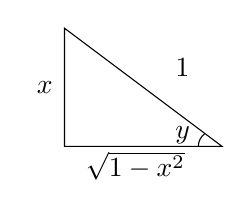
\begin{tikzpicture}[scale=0.5]
\draw (0,0)--(4,0)--(0,3)--cycle;
\draw (3.0,.28) node{$y$};
\draw (3.4,0) arc (180:127:4mm);
\draw (-.5,1.5) node{$x$};
\draw (1.8,-.5) node{$\sqrt{1-x^2}$};
\draw (3,2) node{$1$};
\end{tikzpicture}}
}
%
\SetQuestion{
\unote{Example~\eref{text}{eg_2_12_2}}
\[y=\arctan x\] Find $\diff{y}{x}$.}
\SetAnswer{\unote{Example~\eref{text}{eg_2_12_2}}\color{answercolor}\small
\begin{align*}
y(x)&=\arctan x\\
x&=\tan y(x)\\
\diff{}{x}[x]&=\diff{}{x}[\tan y(x)]\\
1&=\sec^2 y(x) \cdot \diff{y}{x}(x)\\
\diff{y}{x}(x)&=\cos^2 y(x)\\
\diff{y}{x}(x)&=\left(\frac{\text{adj}}{\text{hyp}}\right)^2
=\left(\frac{1}{\sqrt{1+x^2}}\right)^2\\
&=\frac{1}{1+x^2}
\end{align*}
\smash{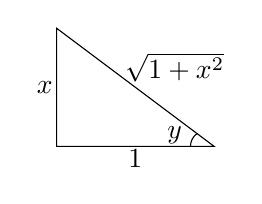
\begin{tikzpicture}[scale=0.5]
\draw (0,0)--(4,0)--(0,3)--cycle;
\draw (3.0,.28) node{$y$};
\draw (3.4,0) arc (180:127:4mm);
\draw (-.3,1.5) node{$x$};
\draw (2,-.3) node{$1$};
\draw (3,2) node{$\sqrt{1+x^2}$};
\end{tikzpicture}}}
%
\SetQuestion{
\unote{Example~\eref{text}{eg_2_12_1}}
\[y=\arccos x\]
Find $\diff{y}{x}$.}
\SetAnswer{\unote{Example~\eref{text}{eg_2_12_1}}
\color{answercolor}\small
\begin{align*}
y(x)&=\arccos x\\
x&=\cos y(x)\\
\diff{}{x}[x]&=\diff{}{x}[\cos y(x)]\\
1&=-\sin y(x) \cdot \diff{y}{x}(x)\\
\diff{y}{x}(x)&=\frac{-1}{\sin y(x)}\\
\diff{y}{x}(x)&=\frac{-\text{hyp}}{\text{opp}}
=\frac{-1}{\sqrt{1-x^2}}
\end{align*}

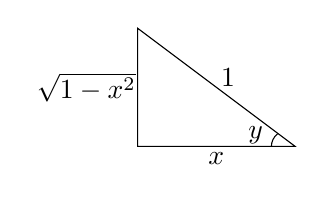
\begin{tikzpicture}[scale=0.5]
\draw (0,0)--(4,0)--(0,3)--cycle;
\draw (3.4,0) arc (180:127:4mm);
\draw (3.0,.28) node{$y$};
\draw (-1.3,1.5) node{$\sqrt{1-x^2}$};%opp
\draw (2,-.3) node{$x$};%adj
\draw (2.3,1.75) node{$1$};%hyp
\end{tikzpicture}}

\end{QuestionSet}
\end{frame}
%----------------------------------------------------------------------------------------
%------------------------------------------------------------------

\begin{frame}[t]
\only<1-2>{\AnswerYes}
\unote{Example~\eref{text}{eg_2_12_3}}
To differentiate arcsecant, arccosecant, and arccotangent, you can use the chain rule!\pause

\color{answercolor}
\[\diff{}{x}\left[ \text{arccsc}(x)\right]=\diff{}{x}\left[\arcsin\left(\frac{1}{x}\right)\right]=\diff{}{x}\left[\arcsin\left(x^{-1}\right)\right]\]\pause


\answer{\footnotesize\begin{align*}
\diff{}{x}&\left[\arcsin\left(\boxed{x^{-1}}\right)\right]=
\frac{1}{\sqrt{1-\left(\boxed{x^{-1}}\right)^2}}\cdot\boxed{\left( -x^{-2}\right)}
=\frac{-1}{x^2\sqrt{1-x^{-2}}}\\
&=\frac{-1}{\sqrt{x^4}\sqrt{1-x^{-2}}}
=\frac{-1}{\sqrt{x^2}\sqrt{x^2}\sqrt{1-x^{-2}}}
=\frac{-1}{\sqrt{x^2}\sqrt{x^2-1}}
=\frac{-1}{|x|\sqrt{1-x^{2}}}
\end{align*}}
\end{frame}

%----------------------------------------------------------------------------------------
%------------------------------------------------------------------
\begin{frame}
\begin{block}{Derivatives of Inverse Trigonometric Functions -- Theorem~\eref{text}{thm:DIFFinvtrigderiv}}
\begin{multicols}{2}
\color{answercolor}
Memorize:\\[1em]
$\diff{}{x}[\arcsin x] = \dfrac{1}{\sqrt{ 1-x^2}}$\\
$\diff{}{x}[\arccos x] = -\dfrac{1}{\sqrt{ 1-x^2}}$\\
$\diff{}{x}[\arcsin x] = \dfrac{1}{ 1+x^2}$\\
\columnbreak 
\color{black}
Be able to derive:\\[1em]
$\diff{}{x}[\text{arccsc}~ x]=-\dfrac{1}{|x|\sqrt{x^2-1}}$\\
$\diff{}{x}[\text{arcsec}~ x]=\dfrac{1}{|x|\sqrt{x^2-1}}$\\
$\diff{}{x}[\text{arccot}~ x]=-\dfrac{1}{1+x^2}$\\ $ $
\end{multicols}
\end{block}

\end{frame}
%------------------------------------------------------------------